\section{Simulation}

To simulate everything before building the rover the tool Protesu 8\footnote{https://www.labcenter.com/} was used. This powerful tool allows the user to create any circuit and run a HEX file to controll any microcontroller. Scheme from the figure \ref{fig6} was designed in the tool in order to test the configuration and programming of the board.


\begin{figure}[htbp]
    \centerline{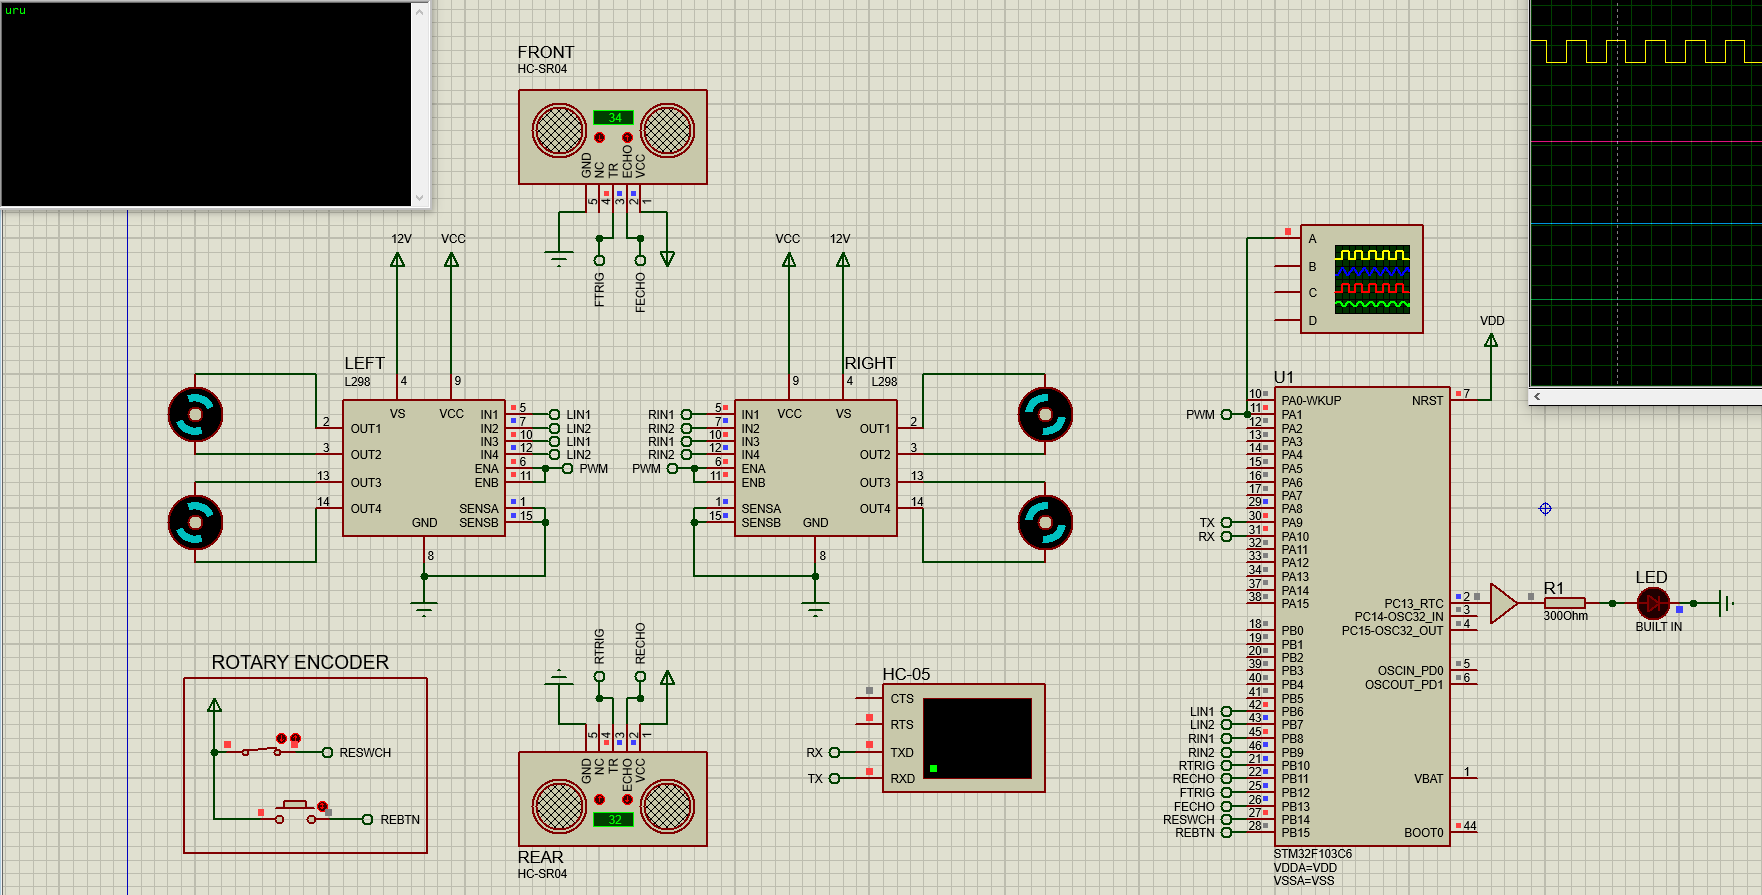
\includegraphics[width=9cm]{Images/Proteus.png}}
    \caption{Proteus simulation}
    \label{fig9}
\end{figure}

This type of simulation also allows for instruments to be used such as the oscilloscope which is utilized to measuer PWM and a simulation of the bluetooth module using a terminal which supports UART serial communication. Once the Keil IDE compiles the code into HEX file it can be uploaded to the chip and the simulation can be started. As there is no rotary encoder one was simulated by using a switch and a button. Values of the ultrasnoic sensors can be altered in the simulation to simulate the movement of the rover. Motors are the only output from the system and the direction in which they move can be observed while the simulation is running.